\documentclass{article}
%\usepackage[margin=0.5in]{geometry}
%\usepackage{titling}
%\usepackage[compact]{titlesec}
\usepackage{fancyhdr} % custom headers
\usepackage{lastpage} % determine the last page for the footer
\usepackage{extramarks} % header footer
\usepackage{graphicx}
\usepackage{float}
\usepackage{url}
\usepackage[pdfborder={0 0 0}]{hyperref}
\usepackage[table]{xcolor}

% margins
\topmargin=-0.45in
\evensidemargin=0in
\oddsidemargin=0in
\textwidth=6.5in
\textheight=9.0in
\headsep=0.25in

% line spacing
\linespread{1.1}

% setup header and footer
\pagestyle{fancy}
\lfoot{Sega Game Gear on a Chip}
\cfoot{}
\rfoot{Page\ \thepage\ of \protect\pageref{LastPage}}
\fancyhead[LE,RO]{\slshape \rightmark}
\fancyhead[LO,RE]{\slshape \leftmark}
\renewcommand\headrulewidth{0.4pt} % size of the header rule
\renewcommand\footrulewidth{0.4pt} % size of the footer rule

% remove indentation from paragraphs
\setlength\parindent{0pt}


\title{
    \vspace{2in}
    \textbf{Sega Game Gear on a Chip}\\
    Design Report
    \vspace{3in}
}
\author{ Max Thrun | Samir Silbak}
\date{Fall 2012}

\begin{document}
\maketitle

\newpage
\tableofcontents
\newpage

\section{Abstract}
The objective of this project is to reimplement the hardware of the
Sega Game Gear (GG) in a Field Programmable Gate Array (FPGA). To do this
each chip in the system will be reimplemented in Verilog based on
official and 3rd party descriptions and specifications on how they operate. This
document details the design functionality and testing metrics that
will be followed during the implementation and execution of our project.

\section{System Overview}
The Sega Game Gear, released in 1991, was Sega's first attempt at a handheld
gaming console. It featured a Zilog Z80 clocked at 3.58MHz, 8KB of system RAM,
16KB of video ram, and a 160x144 pixel resolution screen.

\begin{figure}[!htbp]
\centering
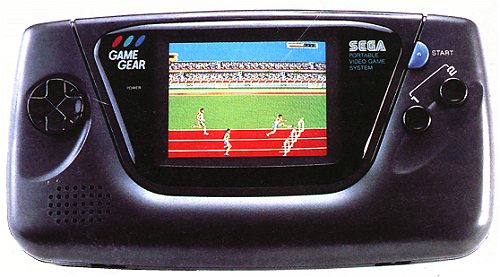
\includegraphics[scale=0.4]{gamegear.png}
\caption{Sega Game Gear \protect\cite{gg}}
\label{fig:gg}
\end{figure}

The image below shows a picture of internal PCB of the Game Gear and
it's major components

\begin{figure}[!htbp]
\centering
\includegraphics[scale=0.4]{gamegear_pcb.png}
\caption{Sega Game Gear PCB}
\label{fig:gg}
\end{figure}

\begin{table}[!htbp]
    \centering
    \begin{tabular}{|c|l|c|l|}
        \hline
        1 & Zilog Z80 CPU           & 4 & 16K VRAM      \\ \hline
        2 & Video Display Processor & 5 & Sega BIOS ROM \\ \hline
        3 & 8K RAM                  & 6 & Controller IO \\
        \hline
    \end{tabular}
\end{table}

\newpage
\subsection{Functional Diagrams}

At a high level the Game Gear can be viewed simply as a system which
takes input from a game controller and produces video and audio has an
output. This description is shown in Figure ~\ref{fig:external}

\begin{figure}[H]
\centering
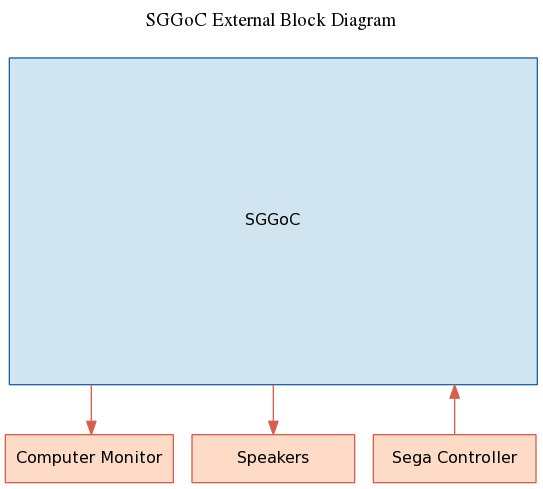
\includegraphics[scale=0.4]{../block_diagrams/block_diagram_external.png}
\caption{Black Box Diagram}
\label{fig:external}
\end{figure}

Internally the functionality can be easily modularized based on the
actual physical components. Additional components will be needed such
as an IO controller and a memory management unit (MMU) to account for 
the lack of tri-state buses in our design (explained later). Figure
~\ref{fig:internal} shows the major functional components in our
design and their interaction with each other.

\begin{figure}[H]
\centering
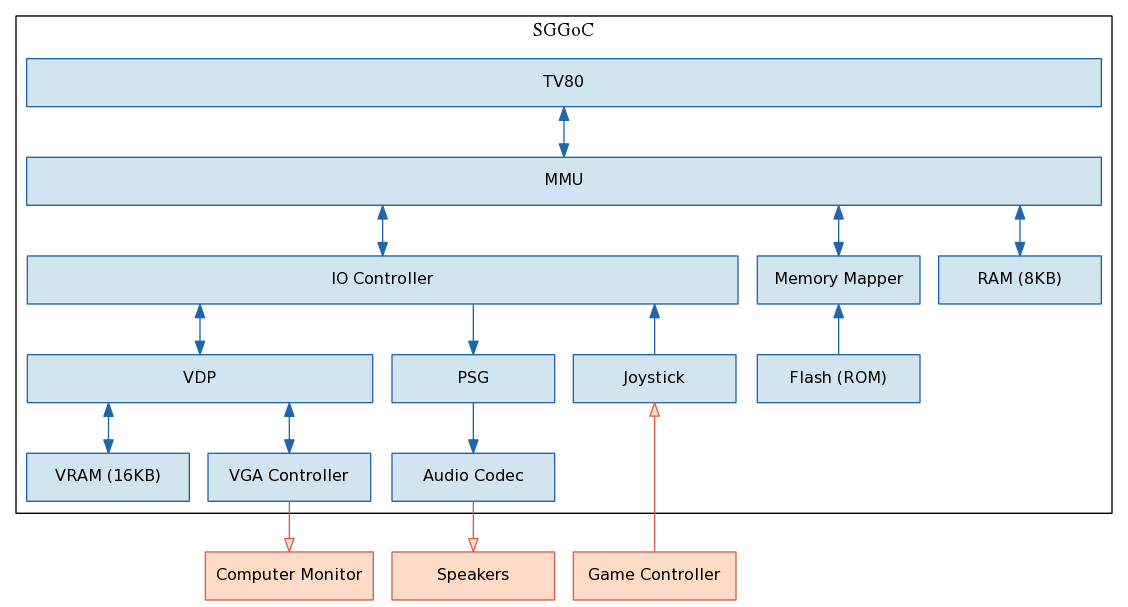
\includegraphics[scale=0.4]{../block_diagrams/block_diagram_internal.png}
\caption{Internal Functional Diagram}
\label{fig:internal}
\end{figure}

\newpage
\section{Cartridges and Memory Mapping}

The Z80 CPU only has 64KB of address space and only 48KB of it is
dedicated to the game cartridge. A "mapper" is used to allow the use of
larger ROMs (as well as on-catridge RAM). Figure ~\ref{fig:gg_cart}
shows a standard GG cartridge and Figure ~\ref{fig:gg_cart_pcb} shows
the internal PCB. The top chip is the Memory Mapper and the bottom chip
is the actual game ROM.

\begin{figure}[!htbp]
    \centering
    \begin{minipage}[!htbp]{0.3\linewidth}
        \centering
        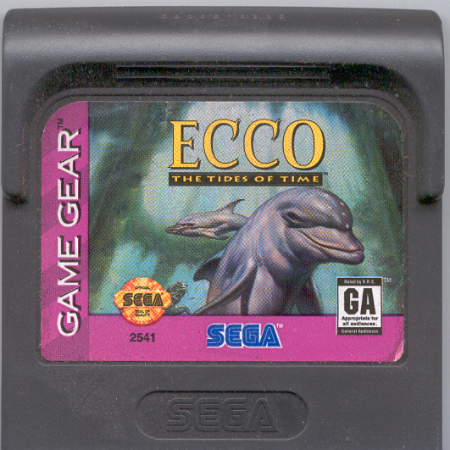
\includegraphics[width=\textwidth]{gg_cart.png}
        \caption{GG Cartridge\protect\cite{gg_cart}}
        \label{fig:gg_cart}
    \end{minipage}
    \hspace{1.5cm}
    \begin{minipage}[!htbp]{0.3\linewidth}
        \centering
        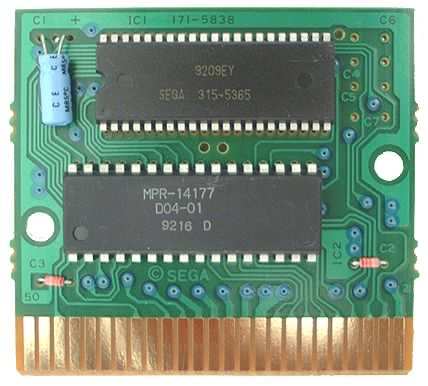
\includegraphics[width=\textwidth]{gg_cart_pcb.png}
        \caption{Cartridge PCB \protect\cite{gg_cart_pcb}}
        \label{fig:gg_cart_pcb}
    \end{minipage}
\end{figure}

\subsection{Sega Mapper}
There are several different mappers in existence but we will only
focus on implementing the "Sega Mapper" as it is the most popular.
The Sega mapper defines 3 16KB slots in the Z80 memory map. Any 16KB bank
of ROM can be mapped into any of these 3 slots. The mapping is
controlled by memory addresses 0xFFFC-0xFFFF.

\begin{table}[!htbp]
    \centering
    \begin{tabular}{|c|c|c|}
        \hline
        \textbf{Control Register} & \textbf{Slot}     & \textbf{Maps to Z80 Address} \\ \hline
        0xFFFC           & Control Bits & -              \\ \hline
        0xFFFD           & 0            & 0x0000-0x3FFF  \\ \hline
        0xFFFE           & 1            & 0x4000-0x7FFF  \\ \hline
        0xFFFF           & 2            & 0x8000-0xBFFF  \\
        \hline
    \end{tabular}
    \caption{Mapper control registers \protect\cite{mapper}}
\end{table}

The ROM is viewed as an array of 16KB banks. The value written into 
the control register determines which bank is selected for 
that slot. Figure ~\ref{fig:mapping_diagram} shows an example of 
how the address space gets mapped to different ROM banks.

\begin{figure}[H]
\centering
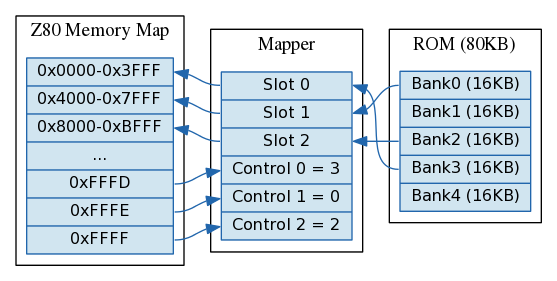
\includegraphics[scale=0.4]{mapper.png}
\caption{Mapping Diagram}
\label{fig:mapping_diagram}
\end{figure}

\subsection{Cartridge Alternatives}
Since we are targeting a standard FPGA development board we cannot
easily use the actual game cartridge without some kind of hardware adaptor.
Additionally, using the actual game cartridge would go
against what we are trying to accomplish with this project which is
eliminating the need for any of the original hardware. Lucky, virtually
every Game Gear cartridge has been dumped and are available online.
Unfortunately, the ROMs range in size all the way up to 4MB and being that
most affordable FPGAs do not have that much block RAM it would be
impossible for us to pack the ROM with the bitstream. A more ideal
solution would be to use a SD card which can be loaded with numerous
ROM files and then write a bootloader to select which one to play.
The complexity of that strategy, however, is not worth the initial
effort. A simpler solution which would allow us to quickly start on the
rest of the project is to load a single ROM file onto the Flash chip
that comes with our DE-1 development board.

\subsection{ROM Flasher}
The technical requirements of interfacing with the flash chip on our board
are outside the scope of our project and as such we will be using
a core provided by Altera \cite{flash_core} to simplify the process.
Figure ~\ref{fig:flash_core} shows the black box diagram of the flash core provided
by Altera.

\begin{figure}[H]
\centering
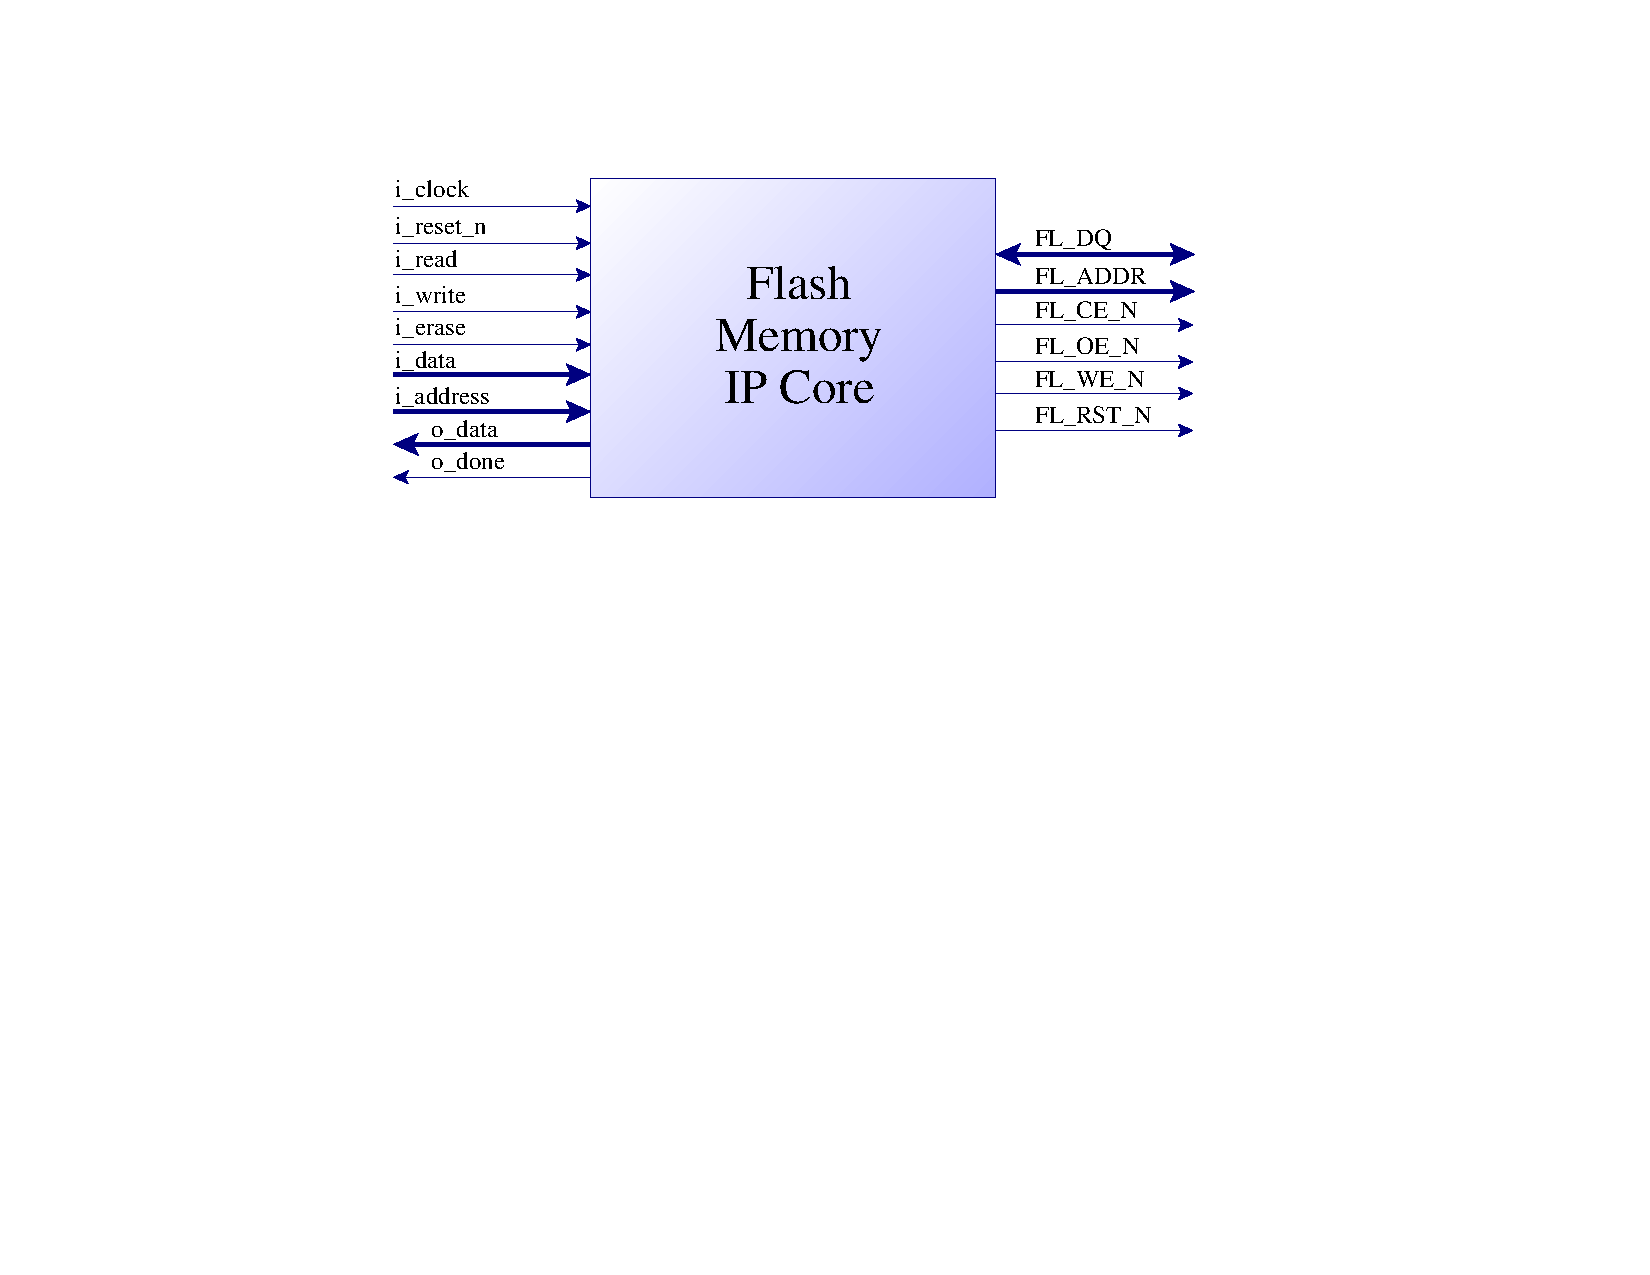
\includegraphics[scale=0.5]{flash_core.pdf}
\caption{Altera Flash Core}
\label{fig:flash_core}
\end{figure}

A "ROM Flasher" project, completely separate from the GG project,
will be used to initially load a single ROM file into the flash chip.
On the computer a Python program will read a ROM file byte by byte
and send it to the FPGA over the serial port. The FPGA will send back
the byte it just recieved as an acknowledgement. Another
Python program will be used to read back and verify that the flash contents
match the ROM file. Figures ~\ref{fig:rom_write} and ~\ref{fig:rom_read} 
illustrate the process of writing and reading a ROM to and from the
flash memory.

\begin{figure}[H]
    \centering
    \begin{minipage}[H]{0.45\linewidth}
        \centering
        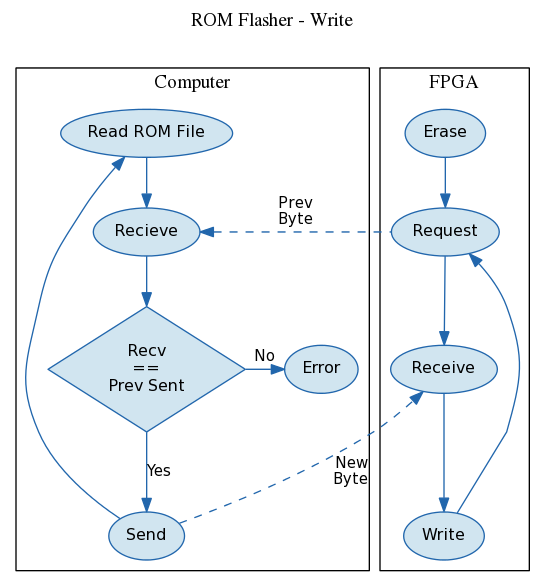
\includegraphics[width=\textwidth]{../../fpga/rom_flasher/doc/block_diagram_write.png}
        \caption{ROM Flasher - Write}
        \label{fig:rom_write}
    \end{minipage}
    \hspace{0.5cm}
    \begin{minipage}[H]{0.45\linewidth}
        \centering
        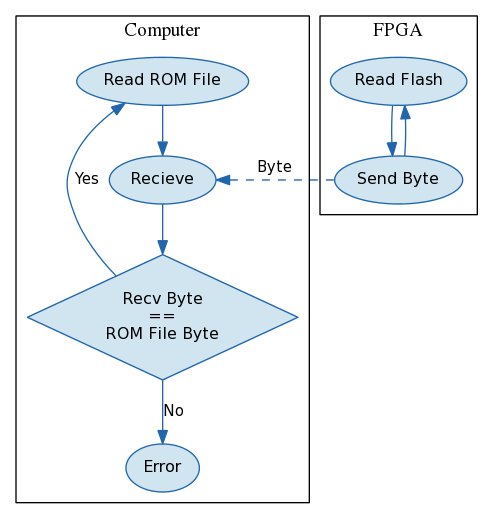
\includegraphics[width=\textwidth]{../../fpga/rom_flasher/doc/block_diagram_read.png}
        \caption{ROM Flasher - Read}
        \label{fig:rom_read}
    \end{minipage}
\end{figure}



\section{Zilog Z80}
The Game Gear uses the classic Zilog Z80 CPU running at 3.58MHz 
as it's main processor.
The re-implementation of the Z80 is completely outside the scope of
this project and as such we will be using the popular TV80 \cite{tv80}
CPU which is a proven, open source, implementation of the Z80
written in Verilog. The interface of the TV80 exactly matches that of
the original Z80, shown in Figure ~\ref{fig:z80}, with the only
exception being the data bus. The original Z80, as well as the whole
Game Gear memory system, relies on tri-state buses where as the TV80 has
a separate bus for data in and data out. 

\begin{figure}[H]
\centering
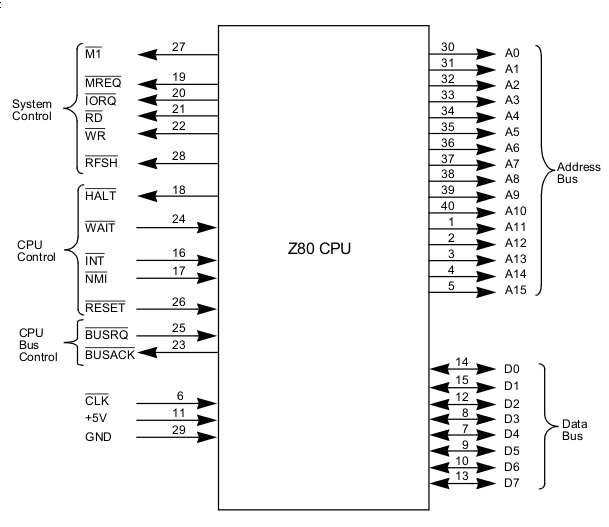
\includegraphics[scale=0.4]{z80.png}
\caption{Zilog Z80}
\label{fig:z80}
\end{figure}

\section{Memory Management Unit (MMU)}
Since our design does not use tri-state buses we cannot simply
connect the data lines from each component together. Instead, we
need to have some kind of memory manager that can multiplex the data
lines to whichever device the address is pointing to according the
system memory map. The full memory map for the Game Gear is shown below

\begin{table}[H]
    \centering
    \fontfamily{pcr}\selectfont
    \begin{tabular}{l|l}
        Address     & Device                           \\
        \hline
        \hline
        0x0000-0x03FF & ROM (unpaged)                    \\ 
        0x0400-0x3FFF & ROM mapper slot 0                \\ 
        0x4000-0x7FFF & ROM mapper slot 1                \\ 
        0x8000-0xBFFF & ROM mapper slot 2 - OR - SaveRAM \\ 
        0xC000-0xDFFF & System RAM                       \\ 
        0xE000-0xFFFF & System RAM (mirror)              \\ 
        0xFFFC       & SaveRAM mapper control           \\ 
        0xFFFD       & Mapper slot 0 control            \\ 
        0xFFFE       & Mapper slot 1 control            \\ 
        0xFFFF       & Mapper slot 2 control            \\
    \end{tabular}
    \fontfamily{}\selectfont
    \caption{Z80 Memory Map \protect\cite{mem_map_table}}
\end{table}

Since the cartridge memory mapper handles the slot mapping itself we are
really only multiplexing between the cartridge and the system RAM.
The system RAM happens to start at a nice edge being that
0xC000 = 0b1100000000000000. To see if we are accessing RAM
we only need to check to see if bits 15 and 16 are high. If so
we can simply use the 13 LSBs of the Z80 address as the index into the RAM. 
This method also accounts for the RAM mirror since the 13 LSBs repeat
starting at 0xE000.

\section{IO Controller}
\section{Video Display Processor (VDP)}
\subsection{Ports}
\subsection{Tiles}
\subsection{CRAM}
\subsection{Layers}
\subsection{Interrupts}
\subsection{Display Timing}
\section{Programmable Sound Generator (PSG)}
\section{VGA Controller}

\newpage
\begin{thebibliography}{9}
    \bibitem{gg} \url{http://mo5.com/musee-machines-gamegear.html}
    \bibitem{gg_cart} \url{http://www.magisterrex.com/prodimages/EccoDolphinGameGear-h450.png}
    \bibitem{gg_cart_pcb} \url{http://www.smspower.org/Development/SMSPagingChips}
    \bibitem{mapper} \url{http://www.smspower.org/Development/Mappers}
    \bibitem{flash_core} \url{ftp://ftp.altera.com/up/pub/flash/altera_up_flash_memory.zip}
    \bibitem{tv80} \url{http://opencores.org/project,tv80}
    \bibitem{mem_map_table} \url{http://code.google.com/p/bizhawk/source/browse/trunk/BizHawk.Emulation/Consoles/Sega/SMS/MemoryMap.Sega.cs}
\end{thebibliography}

\end{document}
